\section{Compressed Sensing Image Reconstruction} \label{cs}
We want to reconstruct an image from under-sampled measurements. We can retrieve the true image if:

\begin{itemize}
	\item we have prior information about the image
	\item measurement space and reconstruction space are incoherent
\end{itemize}

If the interferometer measures sky section which only contains point sources, the objective \eqref{intro:eq:csclean} with the L0 "norm" as prior $p()$ can reconstruct the true image from under-sampled Fourier components. The L0 "norm" is the sum of non-zero elements. The more elements of the image are zero, the lower the regularization term in the objective \eqref{intro:eq:csclean}. This forces the reconstructed image to be sparse, it contains only few non zero elements, or in other words, it assumes the image contains few point sources. 

Let us assume there are $s$ point sources in the image. If we would know the number and location of the $s$ point sources before, we could sample the $s$ pixels to determine their magnitude. Sadly, we do not know the location before in general. The naive approach is therefore to sample at every pixel location. However, this is wasteful: Note that if we land at an empty pixel, the sample gives us almost no new information. If we would sample the whole image pixel for pixel, our average information gain per sample is low. In the under-sampled environment, we only have a limited number of samples available, we want to maximize the information gained for each sample. This is the case when the measurement space is incoherent from the reconstruction space.

Interferometers measure in the Fourier domain, which is maximally incoherent from the image domain. A change in a single pixel will modify all Visibilities, while a change in a single Visibility will modify all pixels. Intuitively, with each sample we now learn information about the $s$ point sources. The average information gain per sample is maximized and we can reconstruct the even from under-sampled measurements. It works because we only need information about the $s$ non-zero pixels.

The question remains, how many samples are needed to reconstruct the image? The answer to that question is an active field of research\cite{candes2011probabilistic}, but depends (among other factors) on the number of non-zero entries in the prior $s$. If the image also contains extended emissions, it increases the number of non-zero pixels $s$, which in turn increases the needed samples. However, if we can represent the image in a more sparse domain, we can reconstruct the image from fewer samples.


\subsection{Sparseland Prior and over-complete Representations}
An image containing both point sources and extended emissions is not sparse in the image domain. When using the L0 "norm" as the prior, we want to reconstruct in a domain where the image can be as sparsely represented as possible. From image compression, we know that natural images tend to be sparse in the Wavelet domain. We can use for example the Haar transform in the prior: $p(x) = \left \| Hx \right \|_0$ and potentially have a more sparse representation.

But why limit the prior to Wavelets? The prior function can be designed as we wish. Wavelets, sine functions or splines together can be used for the reconstruction. In practice many Compressed Sensing applications use a "sparseland" prior \eqref{cs:eq:sparseDic}, a matrix $D$ where each column contains a function potential part of the image. The dictionary matrix $D$ is potentially a large, but has a finite number entries. Any image $x$ we measure consists only of a few entries of $D$. This means the coefficients for the signal parts in the dictionary $\alpha$ are all zero except for $s$ entries for all valid $x$.

\begin{equation} \label{cs:eq:sparseDic}
\begin{split}
x = D \alpha  \qquad  x \in \mathbb{R}^{n}, \alpha \in \mathbb{R}^{m}, D \in \mathbb{R}^{n*m}, \qquad n \leq m \\
\left \| \alpha \right \|_0 = s \qquad s \ll n \leq m
\end{split}
\end{equation}

We can decide with what we fill the columns. Since $D$ can be a mixture of functions and we know point sources are sparse in the image domain, we can use the identity matrix (also sometimes called Dirac basis), which represents single pixel values, and further add columns consisting of wavelets. The number of columns $m$ can be much larger than the number of pixels $n$, which lends itself to over-complete representations.

An over-complete dictionary has more columns than rows (more entries in the dictionary than pixels) and can be used represent an image with even fewer non-zero entries $s$. Starlets\cite{starck2015starlet} and Curvelets\cite{starck2003astronomical} have been developed as over-complete representations for astronomy. In theory, there is no limitation on how many columns we add, but in practice computation power.

Sparseland priors are used with either the L0 "norm" or the L1 norm. The L0 "norm" pushes the objective into non-convex territory. There are specialized optimizers for L0 objectives that approximate the optimum well enough for practical applications. The L0 norm can be relaxed to L1, which results in a convex objective and is practically guaranteed to have the same optimum. In this project, the Gurobi Gurobi\cite{gurobi2018optimizer} optimizer was used with the L1 relaxation.

We could use L2, but what we mostly want in Compressed Sensing Reconstruction is sparsity. 
With that, L0 "norm" is often used. 
The L1 relaxation however is practically guaranteed to have the same minimum as the L0 norm and results in a convex objective function. Since Gurobi works better on the L1 relaxation it was chosen for this project.


\subsection{Choosing the Objective Function} \label{cs:objective}
In general, there are three different reconstruction objectives: The analysis method, where the image $x$ is minimized directly, the synthesis method where the sparse vector $\alpha$ is minimized, or by in-painting the missing Visibilities $V_2$.

\begin{alignat*}{2}
analysis:\qquad \underset{x}{minimize} \:& \left \| I_{dirty} - x \star PSF \right \|_2^2 &&+  \lambda \left \| D^{-1}x \right \|_1 \\
synthesis:\qquad \underset{\alpha}{minimize} \:& \left \| I_{dirty} - D \alpha \star PSF \right \|_2^2 &&+ \lambda \left \| \alpha \right \|_1 \\
in-painting:\qquad \underset{V_2}{minimize} \:& \left \|  I_{dirty} - F^{-1} M V_2 \right \|_2^2 &&+ \lambda \left \| D^{-1}F^{-1}V_2\right \|_1
\end{alignat*}

All three objective functions have the same global minimum. Retrieving $x$ for the analysis objective is trivial. For the second and third objective $x$ can be retrieved by $x = D\alpha$ and by $x = F^{-1}V_2$ respectively. [Empirical and theoretical studies have shown an advantage of the analysis objective over the other two \cite{something}]. However, depending on the measurement space and prior, an objective might become more practical. 

The analysis and in-painting objective require the inverse of the dictionary $D^{-1}$. It exists for orthogonal transformation like the Haar Wavelet transform, but in general does not exist for over-complete dictionaries. For over-complete dictionaries, the Synthesis objective gets used. There are a few notable exceptions like the Starlet Transform, which is both an over-complete representation but also has an inverse $D^{-1}$ defined. Similarly, the in-painting method is useful when the prior is defined as a convolution with the image, since it can be represented as a multiplication in the Fourier domain.During this project, no reconstruction algorithm was found which uses the in-painting method.

So far the data term always featured the deconvolution. 

Data term can also be in the Visibility domain


\subsection{Compressed Sensing Reconstruction Algorithms in Astronomy}
There are already Compressed Sensing implementations for different reconstruction problems. Diverse implementations
\begin{itemize}
	\item PURIFY \cite{purify}
	\item VIS-CS \cite{visCS}
	\item SASIR \cite{girard2015sparse}
\end{itemize}


Purify:
Prior: Mixture of Dirac Basis and Daubechies Wavelets (DB1 - DB8)
Objective: analysis
Optimizer: SDMM
Dirac is a fancy way of saying "it is sparse in pixel space"


\subsubsection{Vis-CS}
Prior: dictionary of gaussians

Objective: Synthesis

Optimizer: Coordinate descent


\subsubsection{SASIR}
Was chosen because it has an inverse. Multiscale effects included in prior.


Prior: Starlets

Multi scale prior,  over complete representation but with a transformation from image space in starlet space.


Objective: synthesis

Optimizer: FISTA

\pagebreak
\subsection{Implementation In CASA}

\begin{wrapfigure}{r}{0.6\textwidth}
	\centering
	\vspace{-15pt}
	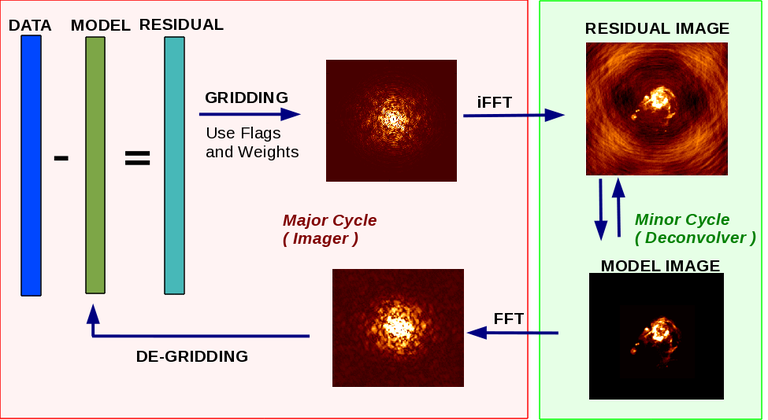
\includegraphics[width=0.9\linewidth]{./chapters/04.cs/img/casa_major_minor.png}
	\caption{Casa Major Minor Cycle. Source \cite{casa2018major}}
	\label{cs:major}
	\vspace{-10pt}
\end{wrapfigure}

The process of reconstructing an image in CASA is split in two separate cycles: The major and the minor cycle. The major cycle transforms the Visibilities to image space and back using the Fourier Transform. The minor cycle is the deconvolution algorithm, which tries to find the true image from a dirty image and a PSF. 

The first major cycle iteration creates the PSF and the dirty image. Then, several minor cycle deconvolve the dirty image. The major cycle then continues and transforms the deconvolved image back to Visibilities. The major cycle ends by calculating the residual Visibilities from the measurements. The next major cycle continues by transforming the residual Visibilities. At the end of several major cycles (and with many, many minor cycle iterations) the model column should contain an approximation of the true visibilities while the residuals should be noise. 


The major and minor cycle separation is built for CLEAN.


In CASA the major cycle is fixed. It was evaluated if it can be modified, but a modification was too time consuming in the context of the project. However CASA allows for the addition of new deconvolution algorithms. 

Major Cycle is expensive.Note that all small field or wide field imaging operations are. Compressed Sensing only needs one


Major cycle is more expensive to compute than a CLEAN minor cylce. 

CLEAN needs potentially many major cycle iterations. A Compressed Sensing Reconstruction would converge to the optimum in one major cylce. Here lies a potential speedup for the Compressed Sensing Reconstruction.

%CASA is a software package built for solving the deconvolution problem for instruments like VLA and ALMA. "Data" Column measurements(calibrated), model column contains the "true" visibilities and the residual column only noise. The architecture is oriented after the CLEAN algorithm, it is split in a major and minor cycle.\ref{cs:major}. The first part of the major cycle produces the dirty image and the PSF. The minor cycle is where a deconvolution algorithm "cleans" the dirty image, several iterations of CLEAN. Major cycle ends with the forward fourier transform. Chi$^2$ approximation of the visibilities.

%The idea of the dirty beam and the clean beam. The output of CASA is the model image convolved with the clean beam plus residuals. Because the model image contains many small peaks, any structure smaller than the clean beam is implausible. Convolving with a gaussian is essentially reducing the resolution. But this is not the case. CLEAN can lead to implausible model images depending on the content: If only a few point sources are visible, clean is plausibe. But for extended emissions clean produces a an area of many peaks which is not true.. With compressed sensing, the ideal prior leads to the true model image. 

%CASA can be extended new deconvolution algorithms, changing minor cycles. During the project it was evaluated if CASA could be modified so wide Field of View imaging can handled by the minor cycle. It was not possible. The implementation is restricted to the deconvolution in the data term. This excludes the in-painting objective function. Or that the data term minimizes on the Visibilities directly.




 
